\section{Introduction}
\label{Chap:Al/Vac:section:Intro}

7000 series Al alloys developed for aerospace applications have high specific strength in the peak-aged condition. Carmakers are exploring options for using stamped 7000 series sheets in structural applications in cars and trucks, from both the manufacturing perspective and the performance perspective. Their widespread implementation in the automotive industry for body and closure applications can achieve lightweight vehicle goals if the challenges of the component forming and fabrication can be overcome\cite{fridlyander2002aluminum,hirsch2011aluminium,hirsch2014recent}.

\begingroup
\begin{figure}[!ht]
  \centering
  \subfigure{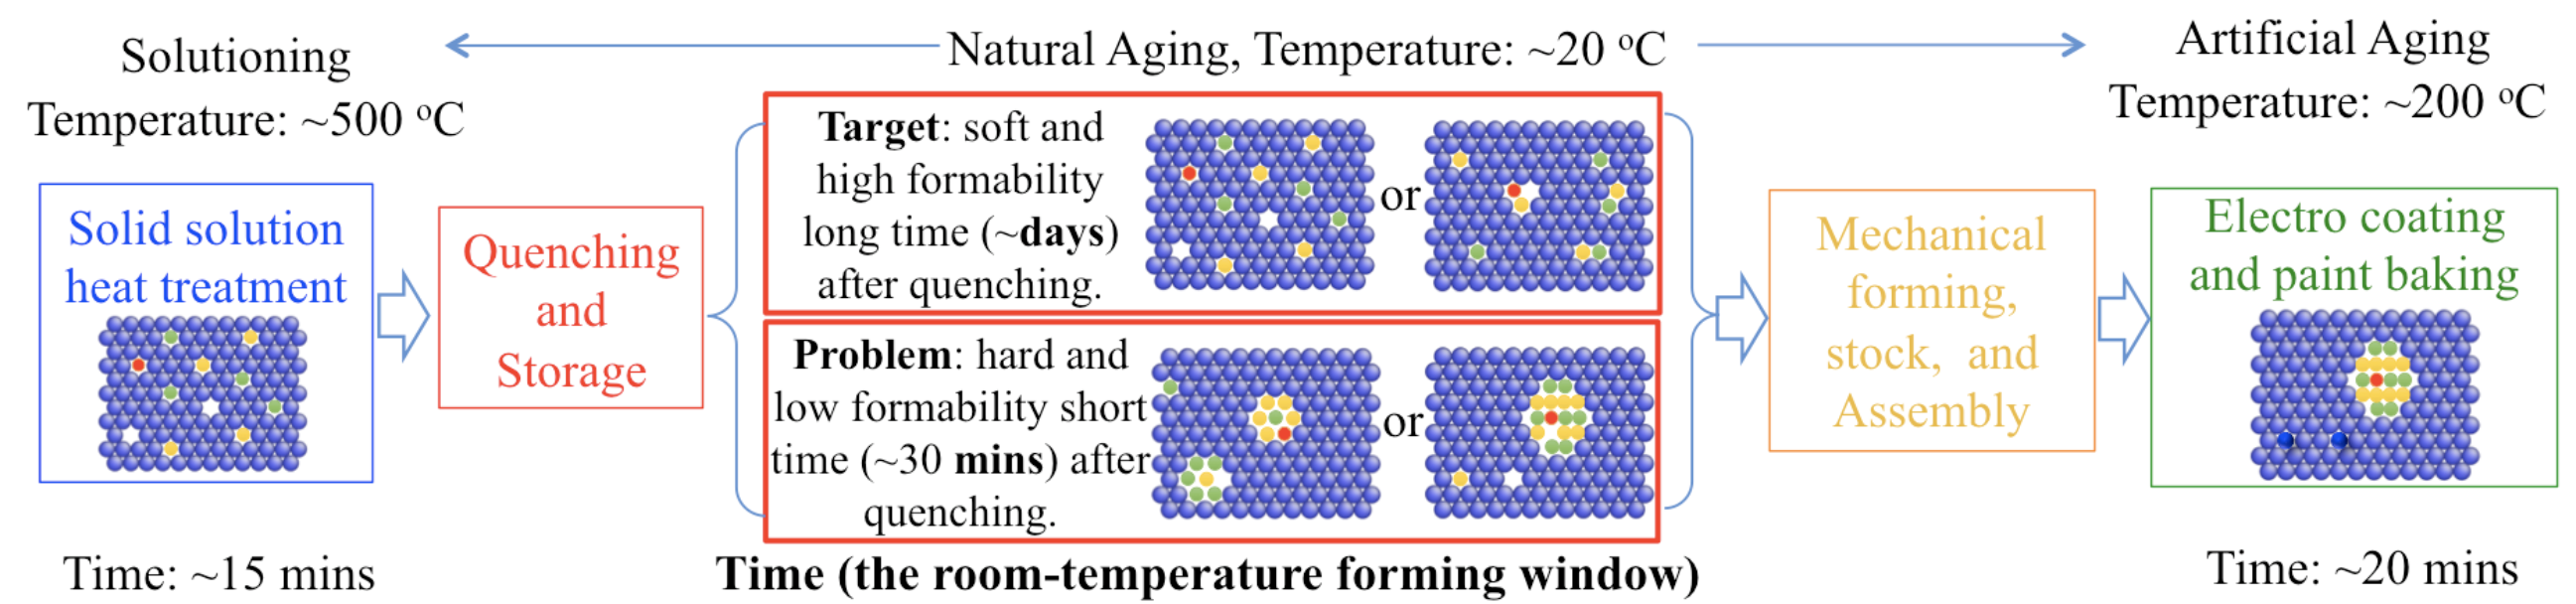
\includegraphics[width=1.0\linewidth]{Chap5/plots/Picture1.png}}
\caption[Schematics of the fabrication process of 7000 series Al sheet alloy parts in the automobile industry.]{Schematics of the fabrication process of 7000 series Al sheet alloy parts in the automobile industry. The corresponding changes of illustrated structures of solute atoms (including clusters and precipitates) during this process are also plotted (blue: Al atoms, other colors: solutes).}
  \label{Chap:Al/Vac:fig1}
\end{figure}
\endgroup

As shown in Figure \ref{Chap:Al/Vac:fig1}, conventional automotive mechanical forming processes, such as stamping and hemming, starts from solid solution heat treatment, then involve room temperature forming of Al sheet alloys in the as-quenched state when alloys have high ductility and formability, and finally followed by artificial aging during the paint bake operation. However, even during the natural aging at room temperatures, the transformation from solid solutions to solute clusters and early-stage precipitates can occur fast  (often within 30 minutes after quenching) for current 7000 series Al alloys. As a result, the formability of these alloys decreases very rapidly and keeps changing as the aging time increases, necessitating costly steps such as warm stamping and coupled solutioning-quenching-stamping operations in a narrow time window\cite{bryant1999effects,li2004biaxial}. These variations of formability and other mechanical properties are all related to the evolution of atomistic structures of precipitates during the sheet processing procedures.

As a result, to understand and to control the nucleation and early stages of precipitation kinetics will have a great impact in automotive applications of age-hardened, light-weight alloys\cite{deschamps1998influence,banhart2011kinetics,liang2012kinetics,deschamps2014precipitation}. The nucleation and growth of precipitates in Al-Zn-Mg-based alloys is currently understood to follow the following sequence: supersaturated solid solution (SSSS) $\rightarrow$ \acf{VRC} $\rightarrow$ \acf{GP} zones (nanoscale coherent Mg/Zn-rich clusters) $\rightarrow$ $\eta'$ (semi-coherent Mg-Zn-Al precipitates with high Zn/Mg ratio) $\rightarrow$ $\eta$ (incoherent $\text{MgZn}_\text{2}$)\cite{ragueneau2000review,deschamps2014precipitation,berg2001gp,chung2018transmission}. During natural aging, the majority of precipitates are \ac{VRC} and \ac{GP} zones, even though $\eta'$ can also be found in some cases\cite{mukhopadhyay1994guinier}. Therefore, in this chapter, how to retard the nucleation and growth of \ac{VRC} and \ac{GP} zones in 7000 series Al alloys during natural aging without reversely effects on the precipitation kinetics during subsequent artificial aging will be focused on. 

Beyond classical theory on the nucleation and early stages of growth of precipitates, atomistic simulations, especially \acf{kMC} simulations, have been applied to investigate the precipitation kinetics in Al alloys\cite{clouet2006kinetic,soisson2010atomistic,soisson1996monte,liang2012kinetics,sha2005kinetic,clouet2004nucleation,vincent2008precipitation,hirosawa1998comparison,sanchez1984generalized}. There simulations were usually conducted to simulate solute atom diffusion based on the vacancy migration in a coherent lattice of the matrix element. Such coherent lattice assumption is still acceptable in our studies of solute clusters and early-stage precipitates. In these \ac{kMC} simulations, the key input is a potential function to describe the activation barrier/energy for the solute/vacancy migration at a particular local lattice occupation environment. For example, the vacancy migration barrier in the pure Al matrix should be different than its counterpart if there is a solute atom occupied the $1^\text{st}$-nearest-neighbor lattice site of the vacancy. Another specific example is shown in Figure \ref{Chap:Al/Vac:barrier}, where the migration barriers for the vacancy jumping to the site \#1, \#2, \#3, and \#4 should be different from each other because these migrations generate distinct change of lattice occupations in the $1^\text{st}$ nearest neighbors of the vacancy.

\begingroup
\begin{figure}[!ht]
  \centering
  \subfigure{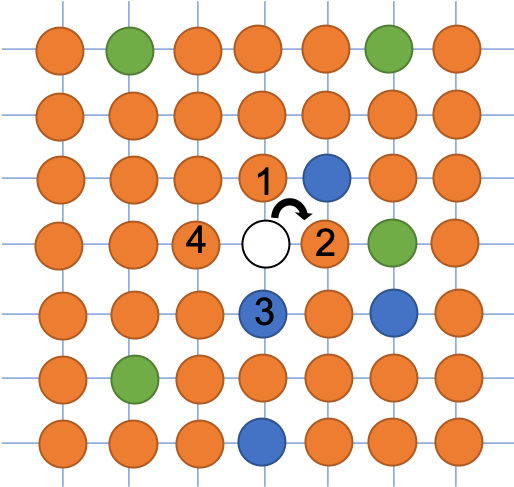
\includegraphics[width=0.5\linewidth]{Chap5/plots/barrier_illustration.png}}
\caption[Illustration of a vacancy migration in a 2D lattice of a multicomponent system.]{Illustration of a vacancy migration in a 2D lattice of a multicomponent system. The orange solid circles represent matrix atoms. Blue and green solid circles represent two different types of solute atoms. The white open circle represents a vacancy. The migration barriers for vacancy jumping to site \#1, \#2, \#3, and \#4 are different based on their $1^\text{st}$ nearest neighbors local environment.}
  \label{Chap:Al/Vac:barrier}
\end{figure}
\endgroup

As we previously mentioned in Section \ref{Chap:Mech:NN}, due to the simplicity of analytical formulas and costly \ac{DFT} calculations, empirical potentials of the vacancy migration barrier usually focus on a limited number of energetic, structural and compositional features in the fitted material systems. As the number of chemical species included in the system increases, it is also getting more difficult to fit the desired empirical potential. For simple vacancy diffusion in bulk lattice or surface diffusion events, \acf{BEP} relationship \cite{bronsted1924katalytische, evans1936further, bell1936theory} was commonly used for calculating the migration barriers of atoms and molecules:
\begin{equation}
\label{Chap:Al/Vac:eq:BEP}
E_a = a \Delta E + b
\end{equation}
where a, b are weighting parameters from fitting, $E_a$ and $\Delta E$ are the migration barrier and the corresponding total energy change due to this migration event, respectively. To further simply the calculations for diffusion in a bulk lattice, researchers used the bond counting model up to a certain cutoff to estimate the total energy change $\Delta E$\cite{soisson1996monte, soisson2010atomistic}. More advanced methods to calculate $\Delta E$ in the coherent lattice include the \acf{CE} formalism that can consider both pair and triple interactions between neighbors \cite{sanchez1984generalized,zunger1994statics,van2001first,persson2010lj,natarajan2016early}. However, most of the \ac{CE} methods only work efficiently for binary or ternary systems due to high computational costs\cite{wu2016cluster}. Even though with some recent development\cite{nguyen2017cluster}, \ac{CE} can predict energy accurately for quinary alloy systems, this method still oversimplified the contribution of atomistic local environments and elastic contributions. Besides, to achieve the same order of accuracy as the number of chemical species increases, the number of parameters needed to fit also increases dramatically\cite{castin2008use}, hence making the computation unaffordable for a long time \ac{kMC} simulations.

Even with correction descriptions of $\Delta E$, we found that the \ac{BEP} relation as Equation \ref{Chap:Al/Vac:eq:BEP} is not valid for the multicomponent alloy systems. As shown in Figure \ref{Chap:Al/Vac:fig2}, the correlation between migration barriers ($E_a$) and energy differences ($\Delta E$) for many vacancy migration events in Al-Mg-Zn systems is far from the linear relation. Here $E_a$ and $\Delta E$ were calculated based on DFT calculations with \acf{CI-NEB}\cite{henkelman2000climbing,henkelman2000improved} in $\sim$1000 cases of vacancy migration in the $4\times4\times4$ supercells of Al fcc lattice with random occupations of Mg/Zn solute atoms. This deviation makes the prediction of accurate vacancy migration barriers very difficult. An inaccurate migration barrier could be fatal in \ac{kMC} models, which is known as the "small-barrier" issue\cite{miron2004multiple}. 


\begingroup
\begin{figure}[!ht]
  \centering
  \subfigure{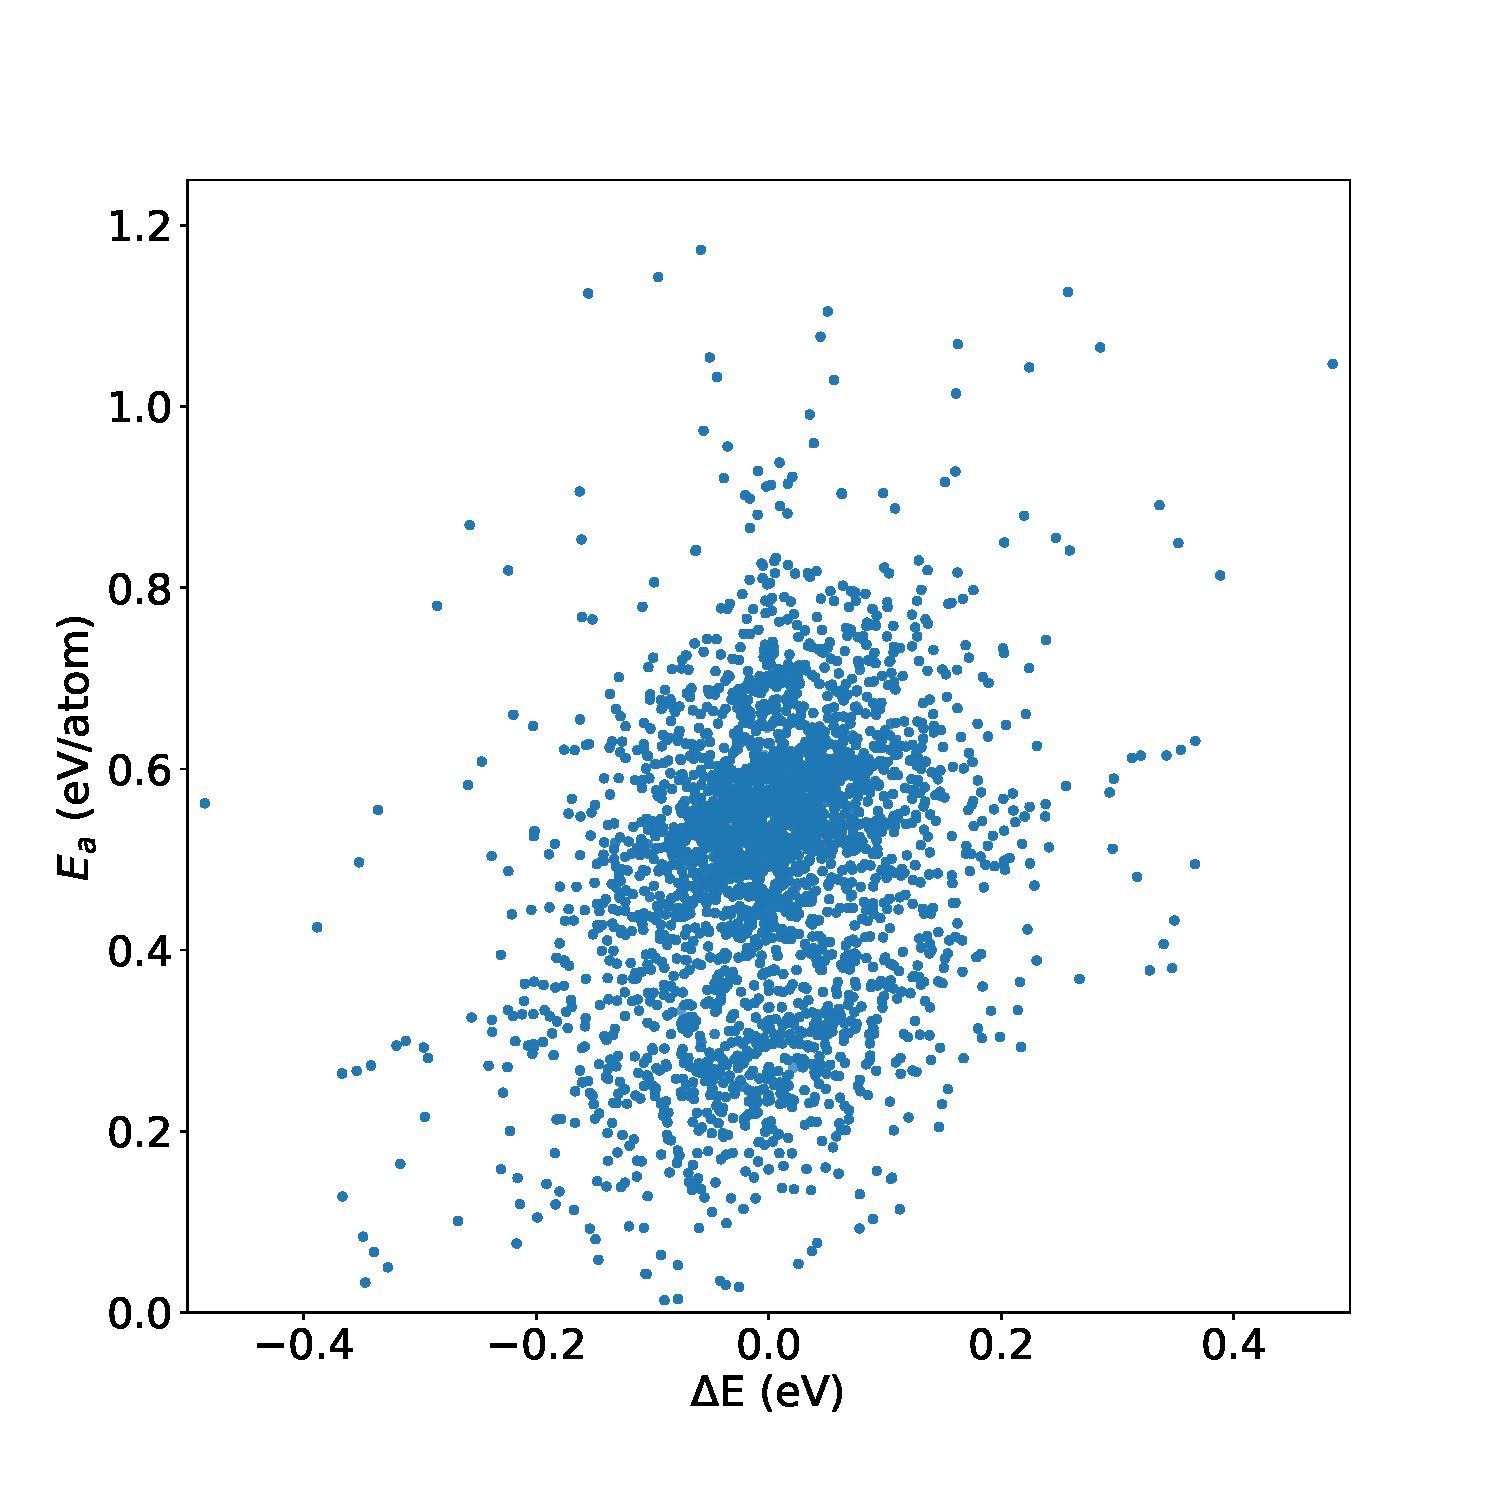
\includegraphics[width=0.8\linewidth]{Chap5/plots/E-EB.pdf}}
\caption[Correlation between migration barriers ($E_a$) and energy differences ($\Delta E$) for many vacancy migration events in Al-Mg-Zn systems.]{Correlation between migration barriers ($E_a$) and energy differences ($\Delta E$) for many vacancy migration events in Al-Mg-Zn systems obtained from our DFT +  \ac{CI-NEB} calculations.}
  \label{Chap:Al/Vac:fig2}
\end{figure}
\endgroup


Thus, we use a machine learning method to predict accurate vacancy migration barriers for multi-component alloy systems in a coherent fcc lattice. Recently statistical machine learning and artificial intelligence techniques start to be used in many research fields, including materials science and engineering. A typical type of applications is to use machine learning to construct the numerical functions for the interatomic force fields \cite{bartok2010gaussian,behler2011atom,szlachta2014accuracy,artrith2016implementation,mehta2014exact,artrith2017efficient}. Compared with conventional interatomic potentials with fixed mathematical forms, the high flexibility of these machine-learning methods increase the possibility to fit complex potential energy landscapes with enough accuracy at the level needed. In this work, we develop a \acf{NN} model to predict vacancy migration barriers using the training data set of thousands of \ac{DFT} calculated barriers for different alloy configurations. 


Then, A \ac{kMC} method based on this \ac{NN} model is developed to study the early transition behavior from a supersaturated solid solution to solute clusters and \acf{GP} zones in Al-Mg-Zn alloys. A local super-basin method  \ref{Chap:Al/Vac:sec:LSKMC}, together with \ac{LRU} cache \ref{Chap:Al/Vac:sec:LRU}, is also implemented to accelerate \ac{kMC} simulations. We also propose a pseudo-atoms approach to efficiently search the alloying strategy to slow down the solute clustering and the corresponding natural aging effects in Al 7000 series alloys. We also develop the quantitative analysis methods to describe the chemical and structural properties of clusters. At last, we propose a machine learning strategy based on the structural and chemical information of clusters and precipitates from \ac{kMC} simulations to predict the cluster strengthening and natural aging effects in future studies.